%
% Documento: GAME DESIGN DOCUMENT
%No PC de casa - o comando está configurado para copiar o arquivo pdf do gdd automaticamente para a pasta da dissertação
%
\documentclass[
oneside,
12pt,                  % Tamanho da fonte
a4paper,               % Tamanho do papel
brazil,                % Idioma
sumario=abnt-6027-2012 % Estilo de sumário conforme ABNT
]{abntex2}

% Codificação e idioma
\usepackage[utf8]{inputenc}
\usepackage[T1]{fontenc}
\usepackage{microtype}
\usepackage{chancery}%Letra cursiva
% Citações ABNT
\usepackage[
alf,
abnt-etal-list=0,
abnt-etal-cite=3,
abnt-etal-text=emph,
abnt-emphasize=bf
]{abntex2cite}


% Figuras e tabelas
\usepackage{graphicx}
\usepackage{booktabs}
\usepackage{multirow, array, makecell, longtable}
\usepackage{caption}
\usepackage{float}

% Fontes e layout
\usepackage{times}
\usepackage{geometry}
\usepackage{indentfirst}
\usepackage{ragged2e}
\usepackage{multicol}

% TikZ e gráficos (para ícones e figuras)
\usepackage{tikz}
\usepackage{pgfplots}
\usepackage{pgf-pie}
\pgfplotsset{compat=1.18}
\usetikzlibrary{calc, patterns, shadows.blur}

% Cores e caixas
\usepackage[dvipsnames]{xcolor}
\usepackage{tcolorbox}
\tcbuselibrary{skins, breakable, theorems, listings, raster}
\usepackage{adjustbox}

% Links e URLs
\usepackage{xurl}
\usepackage{hyperref}

% Citações longas formatadas
\usepackage{quoting}
\quotingsetup{leftmargin=4cm, rightmargin=0cm, font={small}}

\usepackage{graphicx}
\usepackage{xparse} % permite comandos com parâmetros nomeados
\usepackage{xspace}

\usepackage{subfig}
\usepackage{eso-pic}

%%Elementos requisito das tags
\usepackage{tikz}
\usetikzlibrary{shapes.misc} % habilita 'chamfered rectangle'

%%Exibição de códigos
%\usepackage{minted}
%\setminted{ 
%	breaklines=true, 
%	fontsize=\small, 
%	frame=single,
%	breakanywhere=true
%	}

% Configurações de links no PDF
\makeatletter
\hypersetup{
	portuguese,
	colorlinks,
	linkcolor=black,
	citecolor=black,
	filecolor=black,
	urlcolor=black,
	breaklinks=true,
	pdftitle={\@title},
	pdfauthor={\@author},
	pdfsubject={\imprimirpreambulo},
	pdfkeywords={Ecologia; Aprendizagem Baseada em Problemas; Jogo de Plataforma; Investigação científica.}
}
\makeatother

% Formato das legendas
%\DeclareCaptionFormat{myformat}{#1:~#3\par}
%\captionsetup[figure]{format=myformat,font={color=black}}
%\captionsetup[table]{format=myformat,font={color=black}}

% Layout da página
\setlrmarginsandblock{2.5cm}{2.5cm}{*}
\setulmarginsandblock{2.5cm}{2.5cm}{*}
\checkandfixthelayout

\setlength{\parindent}{0pt}
\setlength{\parskip}{1em}
\SingleSpacing

% Novos comandos e ambientes
\newenvironment{bloco}{%
	\medskip
	\setlength{\parskip}{1em}
	\setlength{\parindent}{1.25cm}
	\hrule height 1.5pt
	\medskip
}{}

% Configuração para listas dentro do bloco 
\setlist[itemize]{parsep=0em, itemsep=0em, leftmargin=*, listparindent=\parindent} \setlist[enumerate]{parsep=1em, itemsep=1em, leftmargin=*, listparindent=\parindent}

\newcommand{\gddTitle}[1]{\noindent\textbf{#1}}
\newcommand{\iconize}[1]{\adjustbox{valign=c}{\includegraphics[height=16pt]{./Figuras/#1}}}
\newcommand{\iticonize}[1]{% Melhora o alinhamento vertical
	\adjustbox{raise=-0.3ex}{\includegraphics[height=16pt]{./Figuras/#1}}{ }%
 }
\newcommand{\tituloEsq}[1]{\textbf{\large \underline{#1}}}
\newcommand{\plainref}[1]{\textnormal{\ref{#1}}}

\makeindex



\NewDocumentCommand{\imagemquadro}{O{4cm} O{white} m O{}}{%
	\begin{tcolorbox}[
		title={\strut #4},
		width=#1,
		height=#1,
		colback=#2,
		colframe=black!70,
		boxrule=0.8pt,
		arc=3mm,
		valign=center,
		halign=center,
		nobeforeafter,
		drop shadow={black!40!white},
		before skip=5mm,
		after skip=3mm,
		fonttitle=\scriptsize\centering\color{white},
		colbacktitle=black!50, % cor da tarja
		title filled,          % garante preenchimento
		title style={top=1pt,bottom=1pt}, % <-- reduz espaço interno da tarja
		boxsep=1pt,            % <-- reduz espaço geral interno
		]
		\centering
		\includegraphics[width=0.99\linewidth, keepaspectratio]{./Figuras/#3}
	\end{tcolorbox}%
}



\newcommand{\imagemItem}[2]{\imagemquadro[2cm]{#1}{#2}}%Padrão para imagem de ítens

%Tamnho, endereço da imagem e cor
\newcommand{\imagemPesonagem}[2]{\imagemquadro[3cm][#2]{#1}}%Padrão para imagem de Personagem
\newcommand{\imagemCenario}[2]{\imagemquadro[2cm]{#1}{#2}}%Padrão para imagem de personagens

\newcommand{\newtitle}[2]{\gddTitle{\iconize{#1}\hspace{5px}#2}\addcontentsline{toc}{subsection}{#2}}

\newcommand{\asp}[1]{``#1''\xspace}

\newcommand{\chancerytext}[1]{{\rmfamily\itshape #1}}%Letra cursiva elegante

%%%%%%%%%%%%%% Variáveis a modificar
\newcommand{\nomeGameCompleto}{Araci: Uma Jornada de Resistência e Renovação\xspace}
\newcommand{\nomeGame}{Araci\xspace}
\newcommand{\nomeHeroi}{Araci\xspace}
\newcommand{\nomeOnca}{Yaguareté\xspace}
\newcommand{\nomeReporter}{Anna Harvey\xspace}


\newcommand{\chavePulo}{barra de espaços\xspace}
\newcommand{\chaveSuperpulo}{W\xspace}
\newcommand{\chaveTeleport}{T\xspace}
\newcommand{\chaveChamarPet}{Q\xspace}
\newcommand{\chaveAtaquePet}{P\xspace}
\newcommand{\chaveInformacoes}{I\xspace}

\newcommand{\iconeVida}{\iticonize{"icones/life_icon.png"}}
\newcommand{\iconeEvidencia}{\iticonize{"icones/evidence_icon.png"}}
\newcommand{\iconeSuperpulo}{\iticonize{"icones/superjump_icon.png"}}
\newcommand{\iconeTeleport}{\iticonize{"icones/teleport_icon.png"}}
\newcommand{\iconeFeroz}{\iticonize{"icones/feroz_icon.png"}}
\newcommand{\iconeBluePosion}{\iticonize{"icones/blue_poison_icon.png"}}
\newcommand{\iconeRedPosion}{\iticonize{"icones/red_poison_icon.png"}}
\newcommand{\iconebookPageGreen}{\iticonize{"icones/green_page_book_icon.png"}}
\newcommand{\iconebookPageRed}{\iticonize{"icones/red_page_book_icon.png"}}
\newcommand{\iconeCheckpoint}{\iticonize{"icones/checkPoint_icon.png"}}
\newcommand{\iconeCabure}{\iticonize{"icones/cabure_icon.png"}}
\newcommand{\iconeTotenPass}{\iticonize{"icones/toten_pass_icon.png"}}
\newcommand{\iconeInterruptor}{\iticonize{"icones/interruptor_icon.png"}}
\newcommand{\iconeBotao}{\iticonize{"icones/ok_btn_icon.png"}}

% Comando genérico de tag inline:
\newcommand{\tagbox}[2]{%
	\tikz[baseline=(n.base)]%
	\node[
	chamfered rectangle,
	draw=#2!60!black,
	fill=#2!20,
	text=#2!10!black,
	very thick,
	chamfered rectangle corners={north east,south east}, % opcional: quais cantos chanfrar
	inner xsep=3pt,
	inner ysep=-1pt,
	font=\tiny,
	line width=0.4pt
	] (n) {#1};%
}

\newcommand{\tagPensado}{\tagbox{Pensado}{yellow}\xspace}
\newcommand{\tagPossivel}{\tagbox{Possível}{blue}\xspace}
\newcommand{\tagImplementado}{\tagbox{Implementado}{green}\xspace}
\newcommand{\tagFalha}{\tagbox{Falha}{red}\xspace}
\newcommand{\tagDificuldade}{\tagbox{Dificuldade}{orange}\xspace}

\newcommand{\nomeCidade}{Brasus\xspace}

\usepackage{xargs} % permite parametrização dos comandos

\newcommand{\tamanhoImgsExU}{0.35}%Tamanho da imagem única
\newcommand{\tamanhoImgsExD}{0.25}%Tamanho da imagem dupla
\newcommand{\tamanhoImgsExT}{0.25}%Tamanho da imagem tripla
\newcommand{\tamanhoImgsExQ}{0.25}%Tamanho da imagem Quadrupla

\newcommand{\uimagem}[3][\tamanhoImgsExU]{
\begin{figure}[H]
	\centering
	\includegraphics[height=#1\linewidth]{Figuras/#2}
	\caption{#3}
\end{figure}
}

%O primeiro parâmetro, quando especificado deve ser o valor de #1 Ex. \dimagem[0.3]{imgA.png}{Legenda A}{imgB.png}{Legenda B}
\newcommand{\dimagem}[6][\tamanhoImgsExD]{
	\begin{figure}[H]
		\centering
		 \subfloat[#3]{%
			\includegraphics[height=#1\linewidth]{Figuras/#2}
		}\quad
		\subfloat[#5]{%
			\includegraphics[height=#1\linewidth]{Figuras/#4}
		}
		\caption{#6}
	\end{figure}
}

%O primeiro parâmetro, quando especificado deve ser o valor de #1 Ex. \timagem[0.3]{imgA.png}{Legenda A}{imgB.png}{Legenda B}{imgC.png}{Legenda C}
\newcommand{\timagem}[7][\tamanhoImgsExT]{% 
	\begin{figure}[H] 
		\centering 
		\subfloat[#3]{%
		\includegraphics[height=#1\linewidth]{Figuras/#2} 
		}\quad 
		\subfloat[#5]{%
		\includegraphics[height=#1\linewidth]{Figuras/#4} 
		}\quad 
		\subfloat[#7]{%
		\includegraphics[height=#1\linewidth]{Figuras/#6} 
		} 
	\end{figure} 
		  }

%O primeiro parâmetro, quando especificado deve ser o valor de #1 Ex. \qimagem[0.3]{imgA.png}{Legenda A}{imgB.png}{Legenda B}{imgC.png}{Legenda C}{imgD.png}{Legenda D}
\newcommand{\qimagem}[9][\tamanhoImgsExQ]{% 
	\begin{figure}[H] 
		\centering 
		\subfloat[#3]{%
			\includegraphics[height=#1\linewidth]{Figuras/#2} 
		}\quad 
		\subfloat[#5]{%
			\includegraphics[height=#1\linewidth]{Figuras/#4} 
		}\quad 
		\subfloat[#7]{%
			\includegraphics[height=#1\linewidth]{Figuras/#6} 
		} \quad 
		\subfloat[#9]{%
		\includegraphics[height=#1\linewidth]{Figuras/#8} 
		} 
	\end{figure} 
}
		  
		  
\usepackage{caption}

% Configuração global das legendas
\captionsetup{font=footnotesize}

\newcommand{\linhasnatabela}{
%	\hline
}

%% Cores predefinidas
\definecolor{inimigo1}{HTML}{f9d2d9}
\definecolor{inimigo2}{HTML}{c6938e}
\definecolor{inimigo3}{HTML}{d4574b}

%% Cores predefinidas
\definecolor{personagens}{HTML}{cce8dc}

%Mostra a explicação para quele tópico do GDD
\newcommand{\explique}[1]{
\\\noindent\textit{{\color{gray}\scriptsize #1}\\}
}

%%%%%%%%%%%%%%%%%%%%%%%%%%%%%%%%%%%%%%%%%%%%%%%%%%%%%%
%                CONTEÚDO DO DOCUMENTO
%%%%%%%%%%%%%%%%%%%%%%%%%%%%%%%%%%%%%%%%%%%%%%%%%%%%%%

\begin{document}

% Remove número da página
%\pagenumbering{gobble}


\newpage
\thispagestyle{empty} % sem cabeçalho/rodapé
\ClearShipoutPictureBG

\begin{tikzpicture}[remember picture, overlay]
	% node [opções] at (referência da página) {conteúdo};
	
	\node [
	anchor=south west,    % Alinha o canto inferior esquerdo do texto com a coordenada
	xshift=0.5cm,         % Desloca o texto 1.5cm para a direita
	yshift=0.3cm,         % Desloca o texto 2.0cm para cima
	text=white,          % Define a cor do texto como BRANCO
	font=\bfseries,       % Define a fonte como NEGRITO (bold series)
	] at (current page.south west) {Thiago Lins do Nascimento}; % Conteúdo do texto
\end{tikzpicture}
\AddToShipoutPictureBG*{
	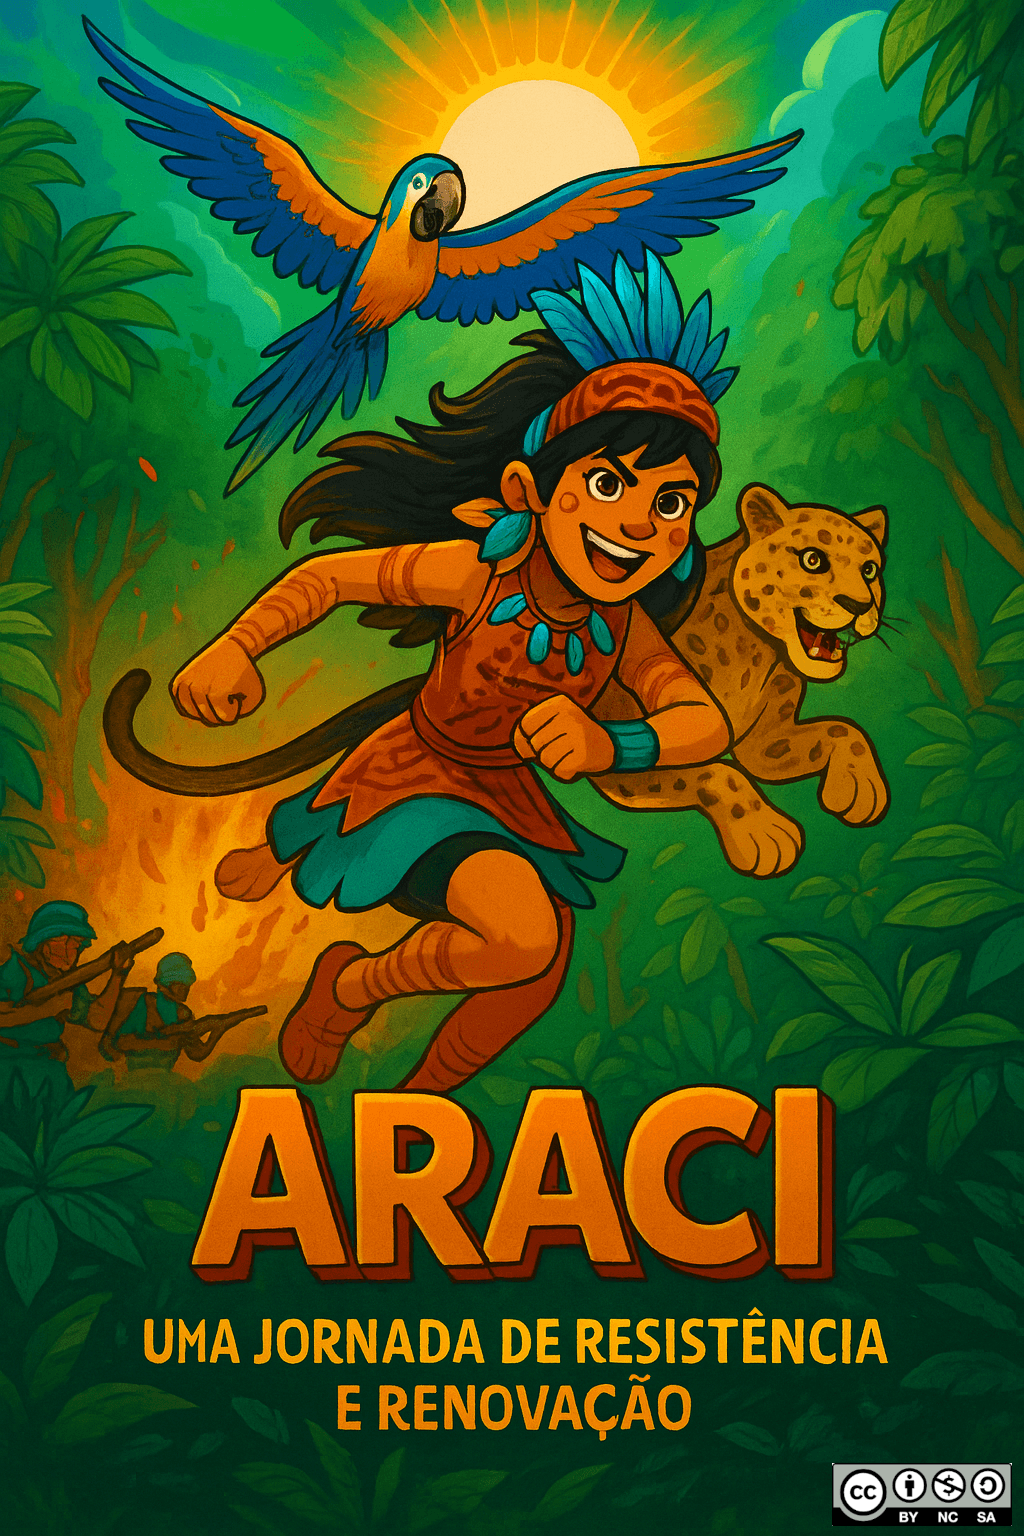
\includegraphics[width=\paperwidth,height=\paperheight]{Figuras/capa1.png}
}
\null % força conteúdo mínimo para shipout
\newpage
\ClearShipoutPictureBG % limpa para não afetar páginas seguintes

% Remove entrada automática "Sumário" no índice
\begingroup
\renewcommand{\addcontentsline}[3]{}
\tableofcontents
\endgroup

	\newpage
%	\setcounter{page}{1}
	\pagestyle{plain}%Página no rodapé
	
	
%	\textbf{\underline{Orientações gerais}}
%	
%	O presente documento acompanhará o desenvolvimento do jogo e, por esse motivo, deverá ser continuamente ajustado e enriquecido ao longo de todo o processo.
%	
%	Além disso, por refletir também o planejamento da criação do jogo -- permitindo a utilização de diferentes plataformas e mecanismos de desenvolvimento -- alguns trechos, especialmente aqueles que envolvem escrita de código ou funcionalidades específicas da engine Godot, poderão ser sinalizados com cinco tipos de tags:
%	
%	\begin{itemize}
%		\item \tagPensado \quad Indica que o recurso ou ação ainda não foi implementado e não há certeza quanto à sua viabilidade;
%		\item \tagPossivel \quad Indica que o recurso ou ação ainda não foi implementado, mas já se sabe que é possível e viável desenvolvê-lo;
%		\item \tagImplementado \quad Indica que o recurso ou ação já está presente na versão atual do jogo;
%		\item \tagDificuldade \quad Indica que o recurso ou ação deveria estar presente na versão atual do jogo, mas encontrou obstáculos em sua implementação;
%		\item \tagFalha \quad Indica que o recurso ou ação já está presente na versão atual do jogo, porém não apresenta o comportamento esperado.
%	\end{itemize}
%	
%	As tags \tagDificuldade e \tagFalha são particularmente relevantes no contexto colaborativo, pois sinalizam problemas já identificados que podem ser resolvidos por voluntários durante o desenvolvimento do projeto.
%	
%	Recursos ou ações que não apresentarem nenhuma tag ainda não foram avaliados quanto à sua viabilidade de implementação ou adequação para uso no jogo.
%	
%	Sugestões, soluções ou dicas serão muito bem vindas e podem ser feitas através da página do projeto no  \href{https://github.com/users/tiagolinsnasc/projects/2}{GitHub} e o projeto ficará disponível (durante todas as etapas de desenvolvimento) em: \href{ https://github.com/tiagolinsnasc/Araci}{Araci}.
%	
%	% Retoma numeração normal
%	\newpage


	\begin{center}
		\textbf{\large Game Design Document (GDD)}
	\end{center}
	\setlength{\parskip}{1em}
	\setlength{\parindent}{1.25cm}
	
	Este documento configura-se como um Game Design Document (GDD) de caráter acadêmico, elaborado com a finalidade de orientar o desenvolvimento de um jogo digital educativo e, simultaneamente, documentar as decisões de design, pedagógicas e técnicas adotadas ao longo do processo. O presente GDD integra a dissertação de mestrado intitulada \textit{Desenvolvimento de um jogo digital para o ensino e aprendizagem de Ecologia no ensino médio} (DOI: 10.5281/zenodo.19581841), constituindo-se como parte do produto educacional vinculado à referida pesquisa. Diferentemente de GDDs estritamente comerciais, este documento incorpora aspectos relacionados aos objetivos educacionais, à intencionalidade pedagógica e à avaliação da aprendizagem, visando sua análise e validação no contexto de pesquisa em educação.
	
	Ao longo deste documento, adota-se uma padronização terminológica com o objetivo de garantir clareza conceitual e consistência na descrição do jogo. O termo ambiente virtual é utilizado para designar o sistema ecológico representado no jogo, enquanto cenário refere-se ao espaço visual e espacial em que ocorrem as interações. A expressão elementos do cenário engloba os componentes presentes no ambiente, sendo elementos interativos aqueles passíveis de ação direta por parte do jogador. O termo mecânicas de jogo refere-se às regras que regulam a relação entre as ações do jogador e as respostas do sistema, enquanto progressão designa o avanço estrutural do jogo ao longo de seus níveis ou etapas. Por fim, o termo jogo é empregado para descrever a experiência do jogador, enquanto projeto ou protótipo funcional são utilizados quando o foco recai sobre o processo e o estágio de desenvolvimento.
	
	Este documento está licenciado sob a licença Creative Commons Atribuição–Não Comercial–Compartilha Igual 4.0 Internacional (CC BY-NC-SA 4.0), permitindo sua reprodução, adaptação e redistribuição para fins não comerciais, desde que atribuída a autoria e mantidos os mesmos termos de licenciamento em eventuais obras derivadas.
	
	O presente trabalho foi realizado com apoio da Coordenação de Aperfeiçoamento de Pessoal de Nível Superior (CAPES)-Brasil-Código de Financiamento 001.
	
	
	
	\newtitle{icoAutor.png}{Autoria}
	\begin{bloco}
		O presente Game Design Document (GDD), bem como o jogo digital nele descrito, constitui produto educacional integrante da dissertação de mestrado intitulada \textbf{Desenvolvimento de um jogo digital para o ensino e aprendizagem de Ecologia no ensino médio}, de autoria de Thiago Lins do Nascimento.
		
		O trabalho foi desenvolvido no âmbito do programa de pós-graduação ao qual a dissertação está vinculada, como requisito parcial para obtenção do título de Mestre, sob orientação formal registrada no documento da dissertação.
		
		A concepção pedagógica, o design do jogo, a implementação das mecânicas, a organização do protótipo funcional, bem como a elaboração deste GDD, são de autoria de Thiago Lins do Nascimento, ressalvados os recursos externos devidamente licenciados e mencionados ao longo do documento.
		
	\end{bloco}
	
	
	\newtitle{icoProjeto.png}{Visão geral do Jogo}
	\begin{bloco}
						
			O jogo proposto é um jogo digital de plataforma em duas dimensões (2D), desenvolvido no motor Godot, voltado para computadores pessoais. O projeto encontra-se em estágio de protótipo funcional, com as principais mecânicas implementadas e em processo de refinamento.
			
			A proposta do jogo baseia-se na exploração de um ambiente virtual inspirado em ecossistemas naturais. Ao longo da progressão, o ambiente reage às ações do jogador, apresentando transformações visuais e funcionais que representam processos de degradação e recuperação ambiental.
			
			O jogador assume o papel de um agente que percorre diferentes áreas do cenário, enfrentando desafios e obstáculos associados, sobretudo, à ação humana sobre o ambiente. A dinâmica do jogo estimula a observação, a tomada de decisões e a compreensão das consequências dessas ações, promovendo uma experiência lúdica baseada na relação entre causa e efeito.
			
			A experiência de jogo privilegia a exploração e a interação com o ambiente, permitindo que o jogador compreenda o funcionamento do ecossistema representado a partir de suas próprias ações. Elementos da fauna e da flora são incorporados como parte integrante da jogabilidade, contribuindo para a construção do significado do ambiente virtual.
			
			Embora o jogo tenha sido concebido para fins educacionais, sua estrutura e mecânicas seguem os princípios do design de jogos digitais, buscando equilíbrio entre desafio, progressão e engajamento. Os fundamentos pedagógicos que orientaram o desenvolvimento do jogo, bem como os objetivos educacionais e os procedimentos de avaliação da aprendizagem, encontram-se detalhados no corpo principal da dissertação à qual este GDD está vinculado.

	\end{bloco}
	
	\newtitle{icoControle.png}{Conceito e Proposta do Jogo}
	\begin{bloco}
		O jogo foi concebido a partir da proposta de representar, em um ambiente virtual interativo, processos relacionados à degradação e à conservação ambiental, utilizando a linguagem dos jogos digitais como meio de engajamento e exploração. O conceito central baseia-se na ideia de que o ambiente não é um cenário estático, mas um sistema dinâmico que responde às ações do jogador.
		
		A proposta do jogo consiste em permitir que o jogador explore diferentes áreas do cenário, observe transformações no ambiente e enfrente desafios que simbolizam impactos ambientais, especialmente aqueles associados à ação humana. Essas transformações são representadas por mudanças visuais, funcionais e de jogabilidade, reforçando a relação entre causa e consequência ao longo da experiência.
		
		Do ponto de vista lúdico, o jogo busca oferecer uma experiência acessível, baseada na exploração, na interação com o ambiente e na progressão gradual por meio de fases ou áreas interligadas. O desafio é construído de forma progressiva, estimulando o jogador a observar o cenário, interpretar sinais visuais e adaptar suas ações conforme as condições do ambiente se modificam.
		
		A proposta narrativa atua como elemento de contextualização, servindo de suporte para a experiência de jogo sem assumir papel central expositivo. O conflito estabelecido entre o jogador e as ameaças presentes no ambiente reforça a temática ambiental e contribui para a construção do significado das ações realizadas durante a jogabilidade.
		
		Embora o jogo tenha finalidade educacional, sua proposta prioriza a integração entre conteúdo e mecânica, evitando a apresentação direta de informações teóricas. O aprendizado pretendido emerge da própria interação com o ambiente e das consequências observadas ao longo da progressão.%, conforme discutido no corpo principal da dissertação.
	\end{bloco}
	
	\newtitle{icoPrototipo.png}{Projeto do Jogo}
	\begin{bloco}
			O projeto do jogo foi desenvolvido com base em decisões de design que buscam equilibrar acessibilidade, engajamento e coerência com a proposta temática apresentada. As escolhas realizadas dizem respeito à estrutura do jogo, ao gênero adotado, ao público-alvo e à forma como a experiência é organizada ao longo da progressão.
		\begin{enumerate}[font=\bfseries]
					
			\item \textbf{Gênero e Estrutura do Jogo:} 
			
			Optou-se pelo gênero plataforma em duas dimensões (2D), com ênfase na exploração do ambiente, por se tratar de um formato amplamente conhecido e de fácil compreensão. Essa escolha favorece a navegação pelo cenário, a observação dos elementos ambientais e a construção gradual da experiência do jogador.
			
			A estrutura do jogo é organizada em fases ou áreas interligadas, permitindo uma progressão gradual. Cada área apresenta desafios específicos e variações no ambiente, estimulando o jogador a adaptar suas ações conforme as condições do cenário se modificam ao longo do jogo.
			
			\item \textbf{Público-alvo:} 
			
			O jogo foi projetado para um público amplo, com foco principal em estudantes do ensino básico, especialmente nos anos finais do ensino fundamental e no ensino médio. Considera-se um público com familiaridade básica com jogos digitais, não sendo exigidas habilidades avançadas, o que contribui para a acessibilidade do jogo em contextos educacionais.
			
			As mecânicas foram pensadas de modo a permitir uma curva de aprendizagem gradual, possibilitando que jogadores com diferentes níveis de experiência compreendam o funcionamento do jogo e avancem progressivamente.
			
			\item \textbf{Decisões de Design:} 
			
			As decisões de design priorizam a interação direta do jogador com o ambiente virtual. O cenário foi concebido como um elemento ativo da jogabilidade, reagindo às ações do jogador por meio de alterações visuais e funcionais que influenciam a progressão.
			
			Elementos de desafio, como obstáculos e ameaças, são utilizados para estimular a exploração e a tomada de decisões, sem comprometer a fluidez da experiência. A progressão no jogo está associada à capacidade do jogador de interpretar o ambiente e agir de forma adequada às situações apresentadas.
			
			\item \textbf{Organização da Experiência do Jogo:}
			
			A experiência de jogo foi estruturada de modo a incentivar a observação e a experimentação. O jogador é constantemente convidado a explorar o ambiente, identificar padrões e compreender as consequências de suas ações ao longo do percurso.
			
			O ritmo do jogo busca equilibrar momentos de desafio e exploração, evitando tanto a sobrecarga de estímulos quanto a repetição excessiva. Essa organização contribui para a manutenção do engajamento e para a clareza da progressão ao longo das fases.
			
		\end{enumerate}
	\end{bloco}
	
	
	\newtitle{icoNarrativa.png}{Narrativa}
	\begin{bloco}
		A narrativa do jogo tem como função principal contextualizar a experiência do jogador e dar sentido às interações realizadas ao longo do jogo. Ela não se apresenta de forma expositiva, mas atua como elemento de suporte, integrando-se ao ambiente e às ações do jogador.
		
		O jogo se passa em um ambiente natural que sofreu alterações decorrentes da ação humana, resultando em processos de degradação que afetam o equilíbrio do ecossistema. Esse cenário serve como pano de fundo para a experiência do jogador, reforçando visual e simbolicamente os desafios enfrentados ao longo da progressão.
		
		\dimagem[0.25]{interface/degradacao}{Visão geral do ambiente inicial do jogo, evidenciando o estado de degradação do cenário.}{interface/gafanhotos}{Os gafanhotos são eliminados após o jogador plantar cinco árvores.}{Exemplos de degradação ambiental e problemas a serem resolvidos.}
		
		O jogador assume o papel de um agente que percorre esse ambiente, interagindo com seus elementos e enfrentando obstáculos que representam diferentes formas de impacto ambiental. Ao longo do jogo, as ações realizadas pelo jogador contribuem para a transformação gradual do cenário, permitindo a visualização de mudanças associadas à recuperação ou à intensificação da degradação ambiental.

		
		A presença de elementos da fauna e da flora desempenha papel importante na construção narrativa, funcionando como indicadores do estado do ambiente e como pontos de interação que orientam o jogador. Esses elementos contribuem para a ambientação do jogo e reforçam o significado das transformações observadas durante a progressão.
		
		\dimagem[0.25]{interface/resgate}{Resgate de animais.}{interface/interacao}{Criação de gado.}{Transformações observadas durante a progressão do jogo.}

		
		O conflito central da narrativa está associado às ameaças que comprometem o equilíbrio do ambiente, frequentemente relacionadas à ação humana. Essas ameaças são representadas por obstáculos e inimigos que surgem ao longo do percurso, funcionando como desafios narrativos e lúdicos que impulsionam a progressão do jogador.
		
		A narrativa evolui de forma integrada à jogabilidade, sem a utilização de longas sequências explicativas. O entendimento do contexto e dos conflitos ocorre principalmente por meio da exploração do ambiente e da observação das mudanças decorrentes das ações realizadas, reforçando a imersão e a coerência entre narrativa e mecânicas de jogo.
			
	\end{bloco}
	
\newtitle{icoEstrutura.png}{Mecânicas do Jogo}
\begin{bloco}
	
	As mecânicas do jogo definem as ações disponíveis ao jogador e as regras que orientam a interação com o ambiente virtual. Elas foram concebidas para garantir fluidez no jogo e coerência com a proposta do jogo, permitindo que o jogador explore o cenário, enfrente desafios e observe as consequências de suas ações ao longo da progressão.
	
	\begin{enumerate}[font=\bfseries]
		\item \textbf{Mecânicas de Movimento} 
	
		As mecânicas de movimento permitem ao jogador deslocar-se pelo ambiente de jogo, explorando diferentes áreas do cenário. O controle do personagem foi projetado de forma simples e responsiva, possibilitando a navegação fluida pelos espaços e a superação de obstáculos distribuídos ao longo das fases.
		
		O deslocamento do jogador é fundamental para a exploração do ambiente e para a interação com os demais elementos do jogo, constituindo a base da experiência de jogabilidade.
		
		
		\uimagem[0.1]{personagens/Araci_corrida}{Movimento de corrida}
		
		\uimagem[0.1]{personagens/Araci_pulo}{Movimento de pulo}
		
		
		\item \textbf{Sistema de Interação com o Ambiente} 
		
		O sistema de interação com o ambiente define as formas pelas quais o jogador pode agir diretamente sobre os elementos do cenário e como essas ações resultam em mudanças no estado do ambiente virtual. Esse sistema constitui um dos eixos centrais da experiência de jogo, uma vez que o ambiente não é tratado como um elemento estático, mas como um componente ativo do jogo.
		
		As interações foram projetadas de modo a serem intuitivas, baseadas principalmente na proximidade do jogador com os elementos do cenário e na observação de sinais visuais que indicam possibilidades de ação.
		
		\begin{enumerate}[label=\arabic{enumi}.\arabic*.]%inicio de subseção
		\item \textbf{Tipos de Elementos Interativos}
		
		\begin{enumerate}[label=\alph*)]
			
			\item Elementos Naturais Interativos
			
			Incluem componentes do cenário associados à fauna e à flora, bem como estruturas naturais do ambiente. Esses elementos podem reagir à presença ou à ação do jogador, funcionando como pontos de interação que influenciam o estado do ambiente ou a progressão no jogo.
			
			\noindent Exemplos de interações incluem:
			
			\begin{itemize}[itemsep=0pt, parsep=0pt]
			\item ativação de elementos naturais;
			\item liberação de caminhos alternativos;
			\item modificação visual do cenário.
			\end{itemize}
			
			
			\dimagem[0.25]{interface/informacoes_laterais01}{Interação do jogador com elemento natural do ambiente}{interface/interacao_elementos_naturais}{Plantio de árvores}{Interação do jogador com elementos naturais.}
			
			\item  Elementos Ambientais Degradados
			
			Esses elementos representam áreas ou estruturas afetadas por processos de degradação ambiental. Sua interação pode resultar tanto em obstáculos adicionais quanto em oportunidades de recuperação do ambiente, dependendo das ações realizadas pelo jogador.
			
			A presença desses elementos reforça a necessidade de observação e tomada de decisão, uma vez que nem todas as interações resultam em benefícios imediatos.
			
			\uimagem[0.3]{interface/estagio05a}{Elemento ambiental degradado presente no cenário. Desgaste do solo pela mineração.}
		
		\end{enumerate}%fim  de a)...
		
		\item \textbf{Estados do Ambiente}
		
		O ambiente do jogo pode apresentar diferentes estados, que refletem seu nível de degradação ou recuperação. Esses estados influenciam diretamente o jogo, alterando a disponibilidade de caminhos, a presença de ameaças e as possibilidades de interação.
		
		\noindent De forma geral, os estados do ambiente podem ser classificados como:
		\begin{itemize}[itemsep=0pt, parsep=0pt]
			\item estado degradado: caracteriza-se pela presença de obstáculos, ameaças e limitação de interações positivas;
			\item estado intermediário: apresenta equilíbrio parcial entre áreas degradadas e recuperadas;
			\item estado recuperado: oferece maior liberdade de exploração e redução de riscos.
		\end{itemize}
		As transições entre esses estados ocorrem em função das ações realizadas pelo jogador ao longo do jogo.
		
		\item \textbf{Regras de Interação e Consequências}
		
		As interações com o ambiente seguem regras claras, permitindo que o jogador compreenda gradualmente as consequências de suas ações. Determinadas interações podem facilitar a progressão, enquanto outras podem intensificar os desafios ou alterar temporariamente o estado do cenário.
		
		\noindent As consequências das interações incluem:
		\begin{itemize}[itemsep=0pt, parsep=0pt]
		\item abertura ou bloqueio de caminhos;
		\item surgimento ou neutralização de ameaças;
		\item alterações visuais que indicam mudança no estado ambiental.
		\end{itemize}
		Essas regras reforçam a relação entre causa e efeito, elemento central da proposta do jogo.
		
		\item \textbf{Feedback Ambiental}
		
		O feedback das interações ocorre principalmente por meio de mudanças visuais no cenário, como variações de cor, animações e transformações nos elementos ambientais. Esse feedback permite que o jogador reconheça rapidamente o impacto de suas ações, sem a necessidade de mensagens explicativas extensas.
		
		O ambiente, dessa forma, atua como um canal de comunicação contínuo entre o jogo e o jogador, orientando a exploração e a tomada de decisões.
		
		\dimagem[.34]{interface/dano_recebido}{Dano recebido ao encostar em um inimigo.}{interface/informacoes_cabure01}{Informações recebidas ao colidir com personagem.}{Exemplos de feedbacks visuais após interação com o ambiente}
		
%		(Inserir Figura X – Exemplo de feedback visual após interação com o ambiente.)
		
		\end{enumerate}%fim  de subseção

		\item \textbf{Sistema de Conflito} 
		
		O sistema de conflito do jogo é responsável por introduzir desafios ao jogador durante a exploração do ambiente, criando situações que exigem atenção, tomada de decisão e adaptação às condições do cenário. Os conflitos foram projetados de modo a integrar-se à proposta temática do jogo, representando ameaças associadas à degradação ambiental e à ação humana sobre o ecossistema.
		
		Os conflitos não têm como objetivo central a eliminação de inimigos, mas a superação de obstáculos e ameaças que comprometem o avanço do jogador e o equilíbrio do ambiente virtual.
		
		\begin{enumerate}[label=\textbf{\arabic{enumi}.\arabic*.}]%inicio de subseção

		\item \textbf{Tipos de Inimigos} 
		
		Os inimigos do jogo são organizados em categorias, de acordo com sua função lúdica e simbólica no ambiente.
		
		\begin{enumerate}[label=\textbf{\alph*)}]
			\item \textbf{Inimigos Ambientais}
			
			Os inimigos ambientais representam consequências indiretas da degradação do ecossistema, como áreas instáveis, elementos naturais corrompidos ou fenômenos adversos. Esses inimigos não possuem comportamento autônomo complexo, atuando como obstáculos persistentes no cenário.
			
			\noindent Sua função principal é:
			
			\begin{itemize}[itemsep=0pt, parsep=0pt]
				\item limitar o deslocamento do jogador;
				\item criar zonas de risco;
				\item incentivar a observação e o planejamento do percurso.
			\end{itemize}
			
			
			\begin{longtable}{>{\centering\arraybackslash}m{3cm}
					>{\centering\arraybackslash}m{3cm}
					>{\centering\arraybackslash}m{3cm}
					>{\centering\arraybackslash}m{3cm}}
				\linhasnatabela
				
				\multicolumn{4}{c}{\raisebox{-5pt}[0pt][0pt]{\textbf{Animais inimigos}}} \\[2ex]
				\linhasnatabela
				\imagemPesonagem{inimigos/animais/african_snail.png}{inimigo1} & \imagemPesonagem{inimigos/animais/cow.png}{inimigo2} & 
				\imagemPesonagem{inimigos/animais/dove.png}{inimigo1} & 
				\imagemPesonagem{inimigos/animais/estorninho.png}{inimigo1}
				\\
				\linhasnatabela
				Caramujo africano & Boi/Vaca & Pombo & Estorninho-europeu (\textit{Sturnus vulgaris}) \\
				\linhasnatabela
				\imagemPesonagem{inimigos/animais/locust.png}{inimigo1} & \imagemPesonagem{inimigos/animais/rat.png}{inimigo1} & 
				\imagemPesonagem{inimigos/animais/wild_boar.png}{inimigo1} & \\
				\linhasnatabela
				Gafanhoto & Rato doméstico & Javali &  \\
				\linhasnatabela
			\end{longtable}
%			(Inserir Figura X – Exemplo de inimigo ambiental presente no cenário.)
			
			\item \textbf{Inimigos Associados à Ação Humana}
			
			Essa categoria de inimigos simboliza intervenções humanas prejudiciais ao ambiente, representadas de forma abstrata ou estilizada. Esses inimigos apresentam comportamento ativo, interagindo diretamente com o jogador durante o jogo.
			
			Eles atuam como agentes de conflito direto, exigindo respostas rápidas e decisões estratégicas por parte do jogador.
			
			\begin{longtable}{>{\centering\arraybackslash}m{3cm}
					>{\centering\arraybackslash}m{3cm}
					>{\centering\arraybackslash}m{3cm}
					>{\centering\arraybackslash}m{3cm}}
				\linhasnatabela
				
				\multicolumn{4}{c}{\raisebox{-5pt}[0pt][0pt]{\textbf{Inimigos de patrulha}}} \\[2ex]
				\linhasnatabela
				\imagemPesonagem{inimigos/drone_controller.png}{inimigo1} & \imagemPesonagem{inimigos/Guarda_mulher.png}{inimigo1} & 
				\imagemPesonagem{inimigos/Madereiro.png}{inimigo1} & 
				\imagemPesonagem{inimigos/mineiro.png}{inimigo1}
				\\
				\linhasnatabela
				Catrina (Controladora de drone) & Elyra Venturin (Guarda) & Konan (Lenhador) & Velasquez (Mineiro) \\
				\linhasnatabela
			\end{longtable}
			
			
			\begin{longtable}{>{\centering\arraybackslash}m{3cm}
					>{\centering\arraybackslash}m{3cm}}
				\linhasnatabela
				
				\multicolumn{2}{c}{\raisebox{-5pt}[0pt][0pt]{\textbf{Disparadores de projéteis}}} \\[2ex]
				\linhasnatabela
				\imagemPesonagem{inimigos/hunter.png}{inimigo2} & \imagemPesonagem{inimigos/Shooter.png}{inimigo2}
				\\
				\linhasnatabela
				Tob Melindroso (Caçador) & Etrom (Atirador) \\
				\linhasnatabela
			\end{longtable}
			
			
%			(Inserir Figura X – Inimigo associado à ação humana em interação com o jogador.)
			
		\end{enumerate}
		
		\item \textbf{Comportamento dos Inimigos} 
		
		Os comportamentos dos inimigos foram definidos de forma a garantir clareza ao jogador e previsibilidade suficiente para o aprendizado das regras do jogo, sem eliminar o desafio.
		
		\noindent Entre os principais comportamentos observados, destacam-se:
		\begin{itemize}[itemsep=0pt, parsep=0pt]
			\item \textbf{Patrulha:} inimigos percorrem trajetórias pré-definidas no cenário, funcionando como obstáculos móveis.
			\item \textbf{Perseguição:} inimigos reagem à proximidade do jogador, deslocando-se em sua direção por um período limitado.
			\item \textbf{Ameaça Ambiental:} inimigos alteram temporariamente o estado do ambiente, criando áreas de risco ou dificultando a progressão.
		\end{itemize}
		
		Esses comportamentos são combinados de forma gradual ao longo do jogo, contribuindo para o aumento progressivo da complexidade dos desafios.
		
		\item \textbf{Interação entre Jogador e Inimigos}
		
		A interação entre o jogador e os inimigos ocorre principalmente por meio do contato direto, da evasão ou da utilização de elementos do ambiente. O jogo privilegia estratégias de desvio e posicionamento, em vez de confrontos baseados exclusivamente em ataque.
		
		\noindent As consequências da interação podem incluir:
		\begin{itemize}[itemsep=0pt, parsep=0pt]
			\item perda de progresso momentâneo;
			\item alteração do estado do ambiente;
			\item necessidade de reiniciar um trecho do percurso.
		\end{itemize}
		
		Essas consequências reforçam a importância da atenção e da adaptação do jogador às condições do cenário.
		\uimagem{interface/interacao_inimigo}{Exemplo de interação entre jogador e inimigo}
%		(Inserir Figura X – Exemplo de interação entre jogador e inimigo.)
		
		\item \textbf{Função do Sistema de Conflito na Progressão}
		
		O sistema de conflito está diretamente relacionado à progressão do jogador no jogo. À medida que o jogador avança, novos tipos de inimigos e comportamentos são introduzidos, ampliando a variedade de desafios.
		
		\noindent Essa progressão contribui para:
		\begin{itemize}[itemsep=0pt, parsep=0pt]
		\item o aumento gradual da dificuldade;
		\item a diversificação da experiência de jogo;
		\item o reforço da relação entre ações do jogador e transformação do ambiente.
		\end{itemize}
		
		\end{enumerate}%fim da subseção
		
		
		\item \textbf{Power-ups e Elementos de Apoio}
		
		Os power-ups e elementos de apoio do jogo foram concebidos como recursos pontuais que auxiliam o jogador na progressão, sem descaracterizar a proposta central de exploração e interação com o ambiente. Diferentemente de jogos de ação tradicionais, o jogo não utiliza power-ups voltados à proteção direta do personagem ou à neutralização imediata de inimigos.
		
		Os elementos de apoio presentes estão diretamente relacionados à mobilidade do jogador e à recuperação ou transformação do ambiente, reforçando a lógica de que a progressão ocorre principalmente por meio da observação, da adaptação e da interação consciente com o cenário.
		
		\begin{enumerate}[label=\textbf{\arabic{enumi}.\arabic*.}]%Inicio de subseção
			\item \textbf{Tipos de Power-ups}
			
			Os power-ups do jogo são organizados em categorias, de acordo com seu efeito na jogabilidade e sua função dentro do sistema de progressão.
			
		\begin{enumerate}[label=\alph*)]%a)
			
			\item Power-ups de Mobilidade
			
			Os power-ups de mobilidade ampliam temporariamente as capacidades de deslocamento do jogador, permitindo a superação de obstáculos ambientais e o acesso a áreas que não podem ser alcançadas apenas com as habilidades básicas do personagem.
			
			Esses power-ups não eliminam desafios, mas oferecem novas possibilidades de abordagem dos cenários, incentivando a exploração e o planejamento do percurso.
			
			\noindent Entre os efeitos associados a esse tipo de power-up, destacam-se:

			\begin{itemize}[itemsep=0pt, parsep=0pt]
				\item possibilidade de ataque à distância;
				\item ampliação da altura ou alcance do salto;
				\item transposição de obstáculos.
			\end{itemize}
			
			\dimagem[.3]{interface/powerup}{Power-up do teletransporte}{interface/efeito_animacao_teletransporte}{Efeito que marca a obtenção do superpoder do teletransporte}{Exemplo de power-up de mobilidade coletado pelo jogador}
%			(Inserir Figura X – Exemplo de power-up de mobilidade coletado pelo jogador.)
			
			\item Elementos de Recuperação Ambiental
			
			Os elementos de recuperação ambiental atuam como recursos de apoio vinculados à transformação do cenário e à redução de áreas degradadas. Diferentemente de power-ups tradicionais, esses elementos não afetam diretamente os atributos do personagem, mas modificam o estado do ambiente, criando condições mais favoráveis para a progressão.
			
			\noindent A ativação desses elementos pode resultar em:
			\begin{itemize}
			\item neutralização de áreas de risco ambiental;
			\item alteração visual do cenário, indicando recuperação parcial;
			\item liberação de novos caminhos ou facilitação da exploração.
			\end{itemize}
			Esses elementos reforçam a relação entre as ações do jogador e as mudanças observadas no ambiente virtual, alinhando jogabilidade e temática ambiental.
			
%			\uimagem[0.05]{icones/embauba_seed}{}
			\uimagem[0.15]{itens/tree_planted}{Quadros de animação de árvore plantada (Embaúba).}
			
			
%			(Inserir Figura X – Ativação de elemento de recuperação ambiental no cenário.)
			
		\end{enumerate}
		
		\item\textbf{ Condições de Obtenção e Uso}
		
		Os power-ups e elementos de apoio são obtidos por meio da exploração do ambiente e da interação com elementos específicos do cenário. Sua disponibilidade é controlada de modo a evitar uso excessivo e garantir equilíbrio na progressão do jogo.
		
		O uso desses recursos é temporário ou condicionado a regras específicas do ambiente, incentivando o jogador a empregá-los de forma estratégica, conforme os desafios apresentados em cada trecho do jogo.
		
		
		\item \textbf{Relação com Progressão e Dificuldade}
		
		A introdução dos power-ups e elementos de apoio ocorre de forma gradual, acompanhando o aumento da complexidade dos desafios ambientais e dos conflitos presentes no jogo. À medida que o jogador avança, esses recursos passam a atuar como facilitadores pontuais, sem eliminar a necessidade de atenção e adaptação às condições do cenário.
		
		Essa abordagem contribui para a construção de uma curva de dificuldade equilibrada, mantendo o engajamento do jogador e a coerência com a proposta do jogo.
		
		\end{enumerate}%fim de subseção
		
		\end{enumerate}
	\end{bloco}

	
	\newtitle{icoInterface.png}{Interface e Feedback ao Jogador}
	\begin{bloco}
		A interface do jogo foi concebida como um sistema de mediação entre o jogador e o ambiente virtual, fornecendo informações essenciais para a tomada de decisão sem comprometer a imersão. As escolhas de interface priorizam a leitura do ambiente e o uso de sinais visuais integrados ao cenário, reduzindo a dependência de elementos informativos explícitos.
		\begin{enumerate}[font=\bfseries]
			
			\item \textbf{Estrutura Geral da Interface} 
			
			A interface é composta por um conjunto mínimo de elementos visuais persistentes, organizados de forma a não obstruir a visualização do cenário. A maior parte das informações relevantes ao jogador é comunicada por meio do próprio ambiente e de alterações visuais nos elementos do jogo.
			
			Os elementos fixos da interface concentram-se nas bordas da tela, preservando a área central para a exploração e interação.
			
			
			\uimagem[0.5]{interface/plataformas01}{Visão geral da interface durante o jogo.}
%			(Inserir Figura X – Visão geral da interface durante a jogabilidade.)
			
			\item \textbf{Elementos do HUD} 
			
			O HUD (Heads-Up Display) reúne informações essenciais relacionadas ao estado do jogo e à situação do jogador. Esses elementos foram projetados para permitir leitura rápida e compreensão imediata.
			
			\noindent Entre os principais componentes do HUD, destacam-se:
			
			\begin{itemize}
			\item indicadores de progresso;
			\item sinalização de eventos relevantes;
			\item informações relacionadas a estados temporários do jogo.
			\end{itemize}

			O uso de ícones e representações gráficas simples contribui para a clareza e acessibilidade da interface.
			\uimagem[0.45]{interface/HUD_informacoes01}{HUD: Contador de Evidências - canto superior esquerdo; Power-ups habilitados - região superior na área central; Pontos - canto superior direito; Vidas extras - canto inferior esquerdo e Área de informações - canto inferior direito.}
%			(Inserir Figura X – Detalhamento dos elementos do HUD.)
			
			\item \textbf{Sinalização Ambiental}
			
			Grande parte do feedback ao jogador é fornecida por meio de sinalização ambiental, isto é, pistas visuais incorporadas ao próprio cenário. Essas pistas indicam áreas de risco, possibilidades de interação e mudanças no estado do ambiente.
			
			\noindent Exemplos de sinalização ambiental incluem:
			
			\begin{itemize}
			\item variações de cor e iluminação;
			\item animações sutis em elementos interativos;
			\item alterações visuais associadas à degradação ou recuperação ambiental.
			\end{itemize}
			
			Essa abordagem reduz a necessidade de mensagens textuais e favorece a aprendizagem por observação.
			
			\dimagem[0.34]{interface/dinamite01}{Som e pavio queimando reforçam o sinal de perigo.}{interface/buracos}{Buracos escuros e profundos indicam riscos}{Exemplos de sinalização ambiental indicando risco ou interação.}
			
%			(Inserir Figura X – Exemplo de sinalização ambiental indicando risco ou interação.)
			
			\item \textbf{Feedback Visual e Sonoro}
			
			O feedback visual ocorre por meio de animações, efeitos visuais e transformações no cenário que indicam o resultado das ações do jogador. Essas respostas visuais permitem que o jogador reconheça imediatamente se uma ação foi bem-sucedida ou se gerou consequências negativas.
			
			O feedback sonoro atua de forma complementar, reforçando eventos importantes, como interações com o ambiente, surgimento de ameaças ou mudanças no estado do cenário. Os efeitos sonoros foram pensados para serem informativos sem se tornarem excessivos ou repetitivos.
			
			\item \textbf{Comunicação de Risco e Estado do Ambiente}
			
			A interface também desempenha papel fundamental na comunicação de risco e do estado geral do ambiente. Em vez de indicadores numéricos explícitos, o jogo utiliza sinais visuais progressivos que permitem ao jogador inferir o nível de degradação ou recuperação do cenário.
			
			Essa estratégia estimula a atenção ao ambiente e fortalece a relação entre observação, decisão e ação durante o jogo.
			
			\uimagem{interface/estagio03}{Alteração visual que mostra a degradação e invasão do ambiente.}
%			(Inserir Figura X – Exemplo de alteração visual indicando estado ambiental crítico.)
			
		\end{enumerate}
	\end{bloco}
	
	\newtitle{icoProgressao.png}{Sistema de Pontuação e Progressão}
	\begin{bloco}
		O sistema de pontuação do jogo foi concebido como um recurso integrado às mecânicas de jogabilidade, exercendo influência direta sobre determinadas habilidades do personagem. Sua principal função é ampliar gradualmente a capacidade dos superpoderes disponíveis, ao mesmo tempo em que fornece ao jogador um indicativo de desempenho ao longo do jogo. 
		
		A pontuação não constitui o único fator determinante da progressão, mas atua de forma complementar às demais mecânicas, associando o desempenho do jogador a melhorias funcionais nas habilidades do personagem.
		
		A atribuição de pontos ocorre a partir das ações realizadas pelo jogador durante a exploração do ambiente e da superação dos desafios propostos. Essas ações refletem o envolvimento do jogador com o jogo e sua capacidade de interagir de maneira eficaz com o ambiente virtual.
		
		\uimagem[0.25]{interface/pontos_obtidos}{Exemplo de exibição da pontuação durante o jogo.}
		
		\begin{enumerate}[font=\bfseries]
			\item \textbf{Relação entre Pontuação e Progressão} 
			
			A progressão no jogo está vinculada principalmente à exploração do ambiente, à interação com seus elementos e à superação dos obstáculos apresentados. A pontuação atua como um fator de aprimoramento das habilidades do personagem, possibilitando melhorias graduais em mecânicas específicas, sem condicionar de forma rígida o avanço entre áreas ou fases.
			
			De forma específica, o acúmulo de pontos permite o aumento da distância do superpulo em dois níveis distintos, bem como a ampliação do alcance da habilidade de teletransporte. Esses aprimoramentos ampliam as possibilidades de exploração e de abordagem dos desafios, sem eliminar a necessidade de planejamento e observação do ambiente.
			
			Essa abordagem evita a dependência exclusiva de metas numéricas e preserva a fluidez da experiência de jogo, ao integrar progressão funcional e exploração ambiental.
			
			\item \textbf{Função do Sistema de Pontuação}
			
			Além de influenciar diretamente determinadas mecânicas, o sistema de pontuação oferece ao jogador um retorno sobre seu desempenho geral ao longo da partida. Esse retorno contribui para a percepção de progresso e para a compreensão do impacto de suas ações no desenvolvimento da experiência de jogo.
			
			Os dados gerados pelo sistema de pontuação podem ser utilizados, quando pertinente, como indicadores complementares de desempenho, tanto no contexto da jogabilidade quanto em análises associadas ao uso educacional do jogo.
		\end{enumerate}
	\end{bloco}
	
	
	\newtitle{icoDev.png}{Aspectos Técnicos do Desenvolvimento}
	\begin{bloco}
		Este tópico apresenta os principais aspectos técnicos relacionados ao desenvolvimento do jogo, incluindo as ferramentas utilizadas, a organização do projeto e os desafios enfrentados durante a implementação. O objetivo é documentar as decisões técnicas adotadas, sem aprofundar em detalhes excessivos de código.
		
		\begin{enumerate}[font=\bfseries]
			\item \textbf{Ferramentas e Tecnologias Utilizadas} 
			
			O jogo foi desenvolvido utilizando o motor de jogos Godot, escolhido por ser uma ferramenta de código aberto, multiplataforma e amplamente utilizada na comunidade de desenvolvimento de jogos independentes. O uso de software livre contribuiu para a flexibilidade do desenvolvimento e para a adequação do projeto a contextos educacionais.
			
			Além do motor de jogo, foram utilizadas ferramentas auxiliares para a criação e edição de recursos gráficos e para a organização do projeto, respeitando as licenças de uso correspondentes.
			
			\item \textbf{Organização do Projeto} 
			
			A estrutura do projeto foi organizada de forma modular, visando facilitar a manutenção, a expansão e o entendimento do código. Os recursos do jogo, como cenas, scripts e elementos gráficos, foram distribuídos em diretórios específicos, de acordo com sua função no projeto.
			
			Essa organização contribui para a clareza do desenvolvimento e permite a adaptação futura do jogo, seja para a inclusão de novas fases, ajustes nas mecânicas ou melhorias na interface.
			
			
			\uimagem[0.5]{interface/godot_editor}{Projeto no Godot Engine}
%			(Inserir Figura 13 – Exemplo da estrutura geral do projeto no ambiente de desenvolvimento.)
			
			\item \textbf{Implementação das Mecânicas} 
			
			As mecânicas do jogo foram implementadas de modo a garantir responsividade e coerência com a proposta apresentada. O desenvolvimento priorizou a estabilidade do protótipo e a integração entre as diferentes mecânicas, como movimentação, interação com o ambiente, conflitos e progressão.
			
			A implementação foi realizada de forma incremental, permitindo testes constantes e ajustes progressivos ao longo do desenvolvimento.
			
			\item \textbf{Desafios Técnicos e Soluções Adotadas} 
			
			Durante o desenvolvimento do jogo, foram identificados desafios técnicos relacionados à implementação das mecânicas, à organização dos recursos e à integração dos elementos visuais e funcionais. Esses desafios exigiram ajustes na estrutura do projeto e na lógica de funcionamento de determinadas mecânicas.
			
			As soluções adotadas buscaram equilibrar simplicidade e eficiência, garantindo o funcionamento adequado do protótipo e a viabilidade de futuras expansões ou refinamentos do jogo.
			
			\item \textbf{Fontes de Recursos e Materiais Externos}
			
			Os recursos visuais, sonoros e demais materiais empregados no desenvolvimento do jogo foram produzidos pelo autor ou obtidos a partir de fontes externas compatíveis com o uso acadêmico e educacional. Quando utilizados, esses materiais respeitam as condições estabelecidas por suas respectivas licenças, priorizando recursos de domínio público ou licenciados sob termos permissivos.
			
			A utilização de materiais externos ocorreu de forma complementar, sem comprometer a identidade visual e conceitual do jogo. A seleção desses recursos considerou critérios éticos, legais e pedagógicos, de modo a assegurar conformidade com a licença adotada para o projeto e com os princípios da produção acadêmica.
			
			A especificação individual de ferramentas, repositórios ou plataformas de obtenção de recursos não é apresentada neste documento, uma vez que o foco do Game Design Document está na descrição do design e da estrutura do jogo, e não na documentação exaustiva do processo técnico de produção.
			
		\end{enumerate}
	\end{bloco}
	
%	\newtitle{icoPublico.png}{Licenças e Distribuição do Jogo}
%	\begin{bloco}
%	O jogo descrito neste Game Design Document constitui um produto educacional desenvolvido no contexto de uma pesquisa acadêmica, com finalidade didática e formativa. Sua distribuição está associada a contextos educacionais e acadêmicos, podendo ser utilizada em ambientes escolares, projetos de ensino e pesquisas relacionadas ao ensino de ecologia e educação ambiental.
%	
%	O conteúdo do jogo, incluindo sua concepção, mecânicas, narrativa, elementos visuais e documentação associada, está licenciado sob a licença Creative Commons Atribuição-Não Comercial-Compartilha Igual 4.0 Internacional (CC BY-NC-SA 4.0). Essa licença permite a utilização, adaptação e redistribuição do jogo e de seus materiais derivados para fins educacionais e não comerciais, desde que seja atribuída a autoria original e que eventuais obras derivadas sejam licenciadas sob os mesmos termos.
%	
%	
%	
%	A distribuição do jogo pode ocorrer por meio de plataformas digitais, repositórios institucionais ou outros meios compatíveis com a natureza acadêmica do projeto, respeitando-se sempre os termos da licença adotada. O uso comercial do jogo ou de qualquer um de seus componentes não é permitido sem autorização expressa do autor.
%	\end{bloco}

\newtitle{icoPublico.png}{Licenças e Distribuição do Jogo}
\begin{bloco}
	O jogo descrito neste Game Design Document constitui um produto educacional desenvolvido no contexto de uma pesquisa acadêmica, com finalidade didática e formativa. Sua distribuição está associada a contextos educacionais e acadêmicos, podendo ser utilizada em ambientes escolares, projetos de ensino e pesquisas relacionadas ao ensino de ecologia e educação ambiental.
	
	O código-fonte do jogo está licenciado sob a licença MIT (MIT License), permitindo sua utilização, modificação, redistribuição e adaptação, inclusive para fins comerciais, desde que mantida a atribuição de autoria e o aviso de licença original. Essa opção visa favorecer a replicabilidade, a melhoria colaborativa e a ampla adoção do jogo por outros docentes e instituições.
	
	Os demais conteúdos do jogo, incluindo narrativa, concepção pedagógica, mecânicas descritas neste documento, elementos visuais originais, trilha sonora (quando aplicável) e a documentação associada (incluindo este Game Design Document), estão licenciados sob a licença Creative Commons Atribuição–Não Comercial–Compartilha Igual 4.0 Internacional (CC BY-NC-SA 4.0). Essa licença permite a utilização, adaptação e redistribuição desses materiais para fins educacionais e não comerciais, desde que seja atribuída a autoria original e que eventuais obras derivadas sejam licenciadas sob os mesmos termos.
	
	A distribuição do jogo poderá ocorrer por meio de plataformas digitais, repositórios institucionais ou outros meios compatíveis com a natureza acadêmica do projeto, respeitando-se os termos específicos de cada licença aplicável aos diferentes componentes do produto educacional.
\end{bloco}
	
	\newtitle{icoVersao.png}{Considerações Finais do GDD}
	\begin{bloco}
		Este Game Design Document teve como objetivo documentar o projeto e o desenvolvimento de um jogo digital voltado à temática ambiental, apresentando sua visão geral, conceito, narrativa, mecânicas, interface e aspectos técnicos. O GDD foi estruturado de modo a funcionar como um registro técnico do jogo, complementando o corpo principal da dissertação.
		
		O documento reflete o estado atual do jogo, reunindo as principais decisões de design e implementação adotadas ao longo do desenvolvimento. As escolhas descritas visam garantir coerência entre a proposta do jogo, a experiência oferecida ao jogador e a viabilidade técnica do projeto.
		
		O GDD também serve como base para futuras expansões e aprimoramentos do jogo, permitindo ajustes nas mecânicas, na narrativa ou na interface, bem como a inclusão de novos conteúdos ou funcionalidades. Dessa forma, o documento contribui para a continuidade do projeto e para sua possível adaptação a diferentes contextos de uso.
		
		Sugestões, soluções ou dicas serão muito bem vindas e podem ser feitas através da página do projeto no  \href{https://github.com/users/tiagolinsnasc/projects/2}{GitHub} e o projeto ficará disponível (durante todas as etapas de desenvolvimento) em: \href{ https://github.com/tiagolinsnasc/Araci}{Araci}.
		
		
	\end{bloco}
	

	
	
	\noindent\textbf{Links de acesso:}
	\begin{itemize}
		\item Dissertação: \url{https://doi.org/10.5281/zenodo.19581841}
		\item Códigos do jogo: \url{https://github.com/tiagolinsnasc/Araci}
		\item Executáveis do jogo: \url{https://github.com/tiagolinsnasc/Araci/releases/tag/v1.01}
		\item Página do jogo: \url{https://sites.google.com/view/araci-uma-jornada/p%C3%A1gina-inicial}
		\item Este documento (GDD): \url{https://doi.org/10.5281/zenodo.19582151}
	\end{itemize}

	\label{lastGDD}
\end{document}

